\documentclass[11pt, a4paper, english, twoside, notitlepage]{report}

\usepackage{iipr}
\fancyhead[RO, LE]{ }
\fancyhead[LO]{\nouppercase \leftmark}	% Heading on odd pages: Chapter name on the left
\fancyhead[RE]{\nouppercase \rightmark} % Heading on even pages: Section on the right
\fancyfoot[LE,RO]{\thepage} % Roman numbering, foot left on even, foot right on odd pages
\fancyfoot[CE]{Doble Grado en Matem\'aticas e Ingenier\'ia Inform\'atica} %Foot: Center, even pages
\fancyfoot[CO]{Universidad Complutense de Madrid (UCM)} %Foot: Center, odd pages
\renewcommand{\footrulewidth}{0.4pt} % Rule on top of foot
\renewcommand{\headrulewidth}{0.4pt} % Rule below headings
\pagestyle{fancy}

% ________Pruebas________
\usepackage{lipsum}
% _______________________

\usepackage{amsmath}
\begin{document}

\pagenumbering{Alph}
\begin{titlepage}

\title{\huge{\textsc{Complexity Analysis of Polynomial Algorithms}} \\
	\protect
\includegraphics[scale=0.2]{ucm.pdf}}
\author{Ignacio Iker Prado Rujas \\
	Universidad Complutense de Madrid (UCM) \\
	Doble Grado en Matem\'aticas e Ingenier\'ia Inform\'atica}
\date{\today}
\maketitle
\thispagestyle{empty}

\begin{center}
	Tutors: \\
	Jos\'e F. Fernando \textit{\&} J.M. Gamboa \\
	\
\end{center}
	
\begin{abstract}
	This work is about three different proofs of the same fact and a computational comparison between them, looking for the best one.

	Let $R$ be a real closed field and $n\geq 2$. We prove that: (1) for every finite subset $F$ of $R^n$,
	the semialgebraic set $R^n\setminus F$ is a polynomial image of $R^n$; and (2) for any
	independent linear forms $l_1,\dots,l_r$ of $R^n$, the semialgebraic set
	$\{l_1>0,\dots,l_r>0\}\subset R^n$ is a polynomial image of $R^n$.
	
	The key proof here is that $\Qu = \{x > 0, y > 0\}$ is a polynomial image of $\R^2$. This assert is proved in three different ways: a first approach using real algebraic geometry; a second and shorter one, using the composition of 3 rather simple maps; and a third one that applies topology with no computer computations.
	
	(...)
\end{abstract}

\end{titlepage}

\newpage
\mbox{}
\thispagestyle{empty}    % White page
\newpage

\tableofcontents
\thispagestyle{empty}

\newpage
\mbox{}
\thispagestyle{empty}    % White page
\newpage

\begin{chapter}{Polynomial images of $R^n$}
\pagenumbering{arabic}    % Numbering from 1

\begin{section}{Introduction}
	\begin{definition}\label{polyMap}
	Let $R$ be a \hyperref[realCField]{real closed field} and $m, n \in \N_{>0}$. A map $f = (f_1, \dots, f_n): R^m \longrightarrow R^n$ is said to be polynomial if $f_i \in R[x_1, \dots, x_m], i = 1,\dots, n$. 
	\end{definition}
	
	A very famous theorem by Tarski and Seidenberg states:
	\begin{theorem}[Tarski-Seidenberg]\label{tarskiSeidenberg}
	The image of every polynomial map $f: R^m \longrightarrow R^n$ is a \hyperref[semialgSet]{semialgebraic subset} of $R^n$.
	\end{theorem}
	
	In this work we are studying sort of a converse of this statement. In an \emph{Oberwolfach} week \cite{g}, J.M. Gamboa proposed to characterize the semialgebraic subsets of $R^n$ that are polynomial images of $R^m$.
	
	% Comentar lo de los abiertos en relación con la conjetura Jacobiana?
	
	\begin{notation}
	We need to mention to which topology we refer to when we talk about closures, boundaries, etc. More specifically, the \textbf{exterior boundary} of a set $S$ is $\delta S := \overline{S} \setminus S$, with $\overline{S}$ being the \textbf{closure} of $S$ in $R^n$ in the usual topology. $\overline{S}^{\text{zar}}$ is the closure of $S$ with respect to the \hyperref[zariski]{Zariski topology}. $A\subset R^n$ is \textbf{irreducible} if its Zariski closure $\overline{A}^{\text{zar}}$ is an irreducible algebraic set.
	\end{notation}
	
	\begin{subsection}{Necessary conditions and examples}
	To begin working on this idea, we provide some necessary conditions for a set $S\subset R^n$ to be polynomial image of $R^m$. 
	
	It is trivial that for $m = n = 1$ (so $f: R \rightarrow R$), the images of polynomial maps are either a set of one point or singletons (if the map is constant), or unbounded closed intervals (think of $f(x) = x^2$), or the whole $R$ (think of $f(x) = x$).
	
	In the general case, by \hyperref[tarskiSeidenberg]{Tarski-Seidenberg}, $S$ must be a semialgebraic set and, moreover, semialgebraically connected. Even more, by the identity principle for polynomials, $S$ is irreducible and \hyperref[pureDim]{pure dimensional}.
	
	% Añadir el teorema de Shiota y la definición de Nash map?
	
	In the polynomial case there are more constrains.
	
	\begin{definition}
		A polynomial map $f: R^m \longrightarrow R^n$ is said to be \textbf{semialgebraically proper at a point} $p \in R^n$ if there exists an open neighbourhood $K$ of $p$ such that the restriction 
		\begin{align*}
			f^{-1}(K) & \longrightarrow K\\
			x & \longmapsto f(x)
		\end{align*}
		is a \hyperref[properMap]{semialgebraically proper map}.
	\end{definition}
	
	\begin{definition}
		
		A parametric semiline  of $R^n$ is a non-constant polynomial image of $R$.
		
	\end{definition}
	
	It is clear that every parametric semiline is semialgebraically closed, since every polynomial map from $R$ to $R^n$ is semialgebraically proper. Let $\S_f$ denote the set of points $p \in R^n$ at which $f$ is \textbf{not} semialgebraically proper.
	
	\begin{theorem}[Jelonek]\label{jelonek}
		
		Let $f: R^2 \longrightarrow R^2$ be a \hyperref[dominant]{dominant} polynomial map. Then $\S_f$ is a finite union of parametric semilines.
		
	\end{theorem}
	
	With all these ideas in mind, we can get some conclusions in the following proposition:
	
	\begin{proposition}\label{propIntro}
			
	Let $f: R^m \longrightarrow R^n$ be a polynomial map and $S = f(R^m)$.
		\begin{enumerate}[(1)]
			\item $\delta S \subset \S_f$.
				\begin{Proof}
					Suppose $p \in \delta S \setminus \S_f$. Because $p \notin \S_f$, there exists an open neighbourhood $K$ of $p$ such that the restriction $f^{-1}(K) \rightarrow K$ of $f$ is proper, and thus its image $K \cap S$ is a closed subset of $K$. Hence, $p \in K\cap \overline{S} = K \cap (\overline{K\cap S}) = K \cap S$, which yields in a contradiction.
				\end{Proof}
			
			\item Let $m = n = 2$ and $\Gamma$ be a 1-dimensional irreducible component of $\overline{\delta S}^{\text{zar}}$. $\Gamma$ is the Zariski closure of a parametric semiline of $R^2$.
				\begin{Proof}
					Since $f$ is a dominant map, we can apply \hyperref[jelonek]{Jelonek} and get that $\S_f$ is a finite union of parametric semilines, say $M_1, \dots, M_s$ in $R^2$. Then, using (1) we get: $\Gamma \subset \overline{\delta S}^{\text{zar}} \subset \overline{\S_f}^{\text{zar}} = \cup_{i=1}^s  \overline{M_i}^{\text{zar}}$. Lastly, using that both $\Gamma$ and the $\overline{M_i}^{\text{zar}}$'s are irreducible, we must have that for some $i = 1, \dots, s: \Gamma = \overline{M_i}^{\text{zar}}$.
				\end{Proof}
			
			\item Let $p:R^n \rightarrow R$ be a polynomial map which is non-constant on $S$. Then $p(S)$ is unbounded.
				\begin{Proof}
					If $a \in R^m$, let us define $\varphi_a:R \rightarrow R$ as $\varphi_a(t) := p(f(ta))$. Then, $\forall a \in R^m,\ p(S)$ would contain the image $\varphi_a(R):\ \varphi_a(R) \subset p(S)$. Now suppose that $\varphi_a(R)$ is bounded $\forall a$. Then $\varphi_a(R)$ would be a point $r_a$, and given $a, b \in R^m: \ \varphi_a(1) = p(f(ta)) = r_a = \varphi_a(0) = \varphi_b(0) = r_b = p(f(tb)) = \varphi_b(1)$. This implies that $p$ would be constant on $S$, which is a contradiction.
				\end{Proof}
			
		\end{enumerate}
		
	\end{proposition}	
	
	\begin{corolary}
		Because of (3) in proposition \ref{propIntro}, all linear projections of $S$ are either a point or unbounded. Consequently, S is also unbounded or a point.
	\end{corolary}
	
	\begin{example}\label{introExample}
		\
		\begin{enumerate}[(i)]
			
			\item The exterior of the closed unit disc $S = \set{u^2 + v^2 > 1}$ \textbf{is not} a polynomial image of $R^2$. This is because the only irreducible component of $\overline{\delta S}^{\text{zar}}$ is $\set{u^2 + v^2 = 1}$ and this set is not a parametric semiline because it is bounded.
			
			\item Let $S_1 = \set{uv < 1}$ and $S_2 = \set{uv > 1, u > 0}$ (see fig. \ref{fig:introExampleii}).
			They both \textbf{are not} polynomial images of $R^2$ since the Zariski closure of the exterior boundary ($\overline{\delta S_1}^{\text{zar}}$ and $\overline{\delta S_2}^{\text{zar}}$) is the hyperbola $uv = 1$, which is not a parametric semiline.
			
			\begin{figure}[h]
				\begin{subfigure}{.55\linewidth}\centering
					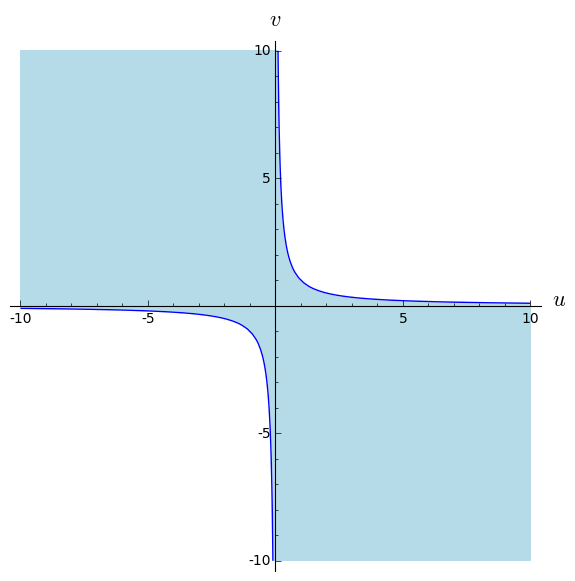
\includegraphics[width=1\textwidth]{plots/ch1_01_S_1.png}
					\caption{$S_1 = \set{uv < 1}$.\label{fig:S_1}}
				\end{subfigure}
				\begin{subfigure}{.55\linewidth}\centering
					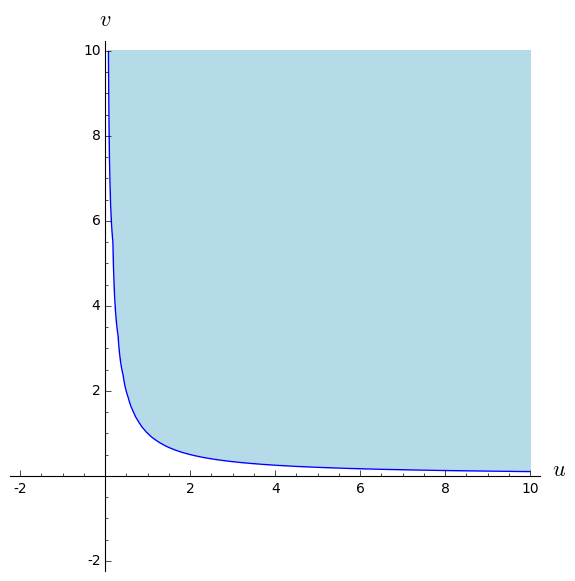
\includegraphics[width=1\textwidth]{plots/ch1_02_S_2.png}
					\caption{$S_2 = \set{uv > 1, u > 0}$.\label{fig:S_2}}
				\end{subfigure}\\[1ex]
				\caption{Plots of the regions defined in example \ref{introExample} (ii).\label{fig:introExampleii}}
			\end{figure}
			
			\item Let $S = R^2 \setminus \set{(0, 0)}$ be the punctured plane. Then $S$ is the image of the polynomial map $(x, y) \mapsto (xy - 1, (xy - 1)x^2 - y)$.
			
			\item Let $\mathbb{H} = \set{v > 0}$ be the open upper half-plane. Then $\mathbb{H}$ is the image of $(x, y) \mapsto (y(xy - 1), (xy - 1)^2 + x^2)$. Furthermore, all the open half-planes are a polynomial image of $R^2$. This is probably the simplest polynomial map whose image is $\mathbb{H}$.
			
		\end{enumerate}
		
	\end{example}
	
	\end{subsection}
	
	\begin{subsection}{Statement of the main results}
	
	Indeed, the main results of this chapter are generalizations of the examples (iii) and (iv) from \ref{introExample}, meaning:
	
	\begin{theorem}\label{finSetTh}
		
		Let $n \ge 2$. For every finite set $F\subset R^n$, the semialgebraic set $R^n \setminus F \subset R^n$ is a polynomial image of $R^n$.
		
	\end{theorem}
	
	\begin{theorem}\label{openQuadGen}
		
		Let $n \ge 2$. For any independent linear forms $l_1, \dots, l_r$ of $R^n$, the open semialgebraic set $\set{l_1>0, \dots, l_r>0}$ is a polynomial image of $R^n$.
		
	\end{theorem}
	
	Before the paper \cite{fg}, the known open sets that are polynomial images of $R^2$ have irreducible exterior boundary, and they are all deformations of $\mathbb{H}$. J.M. Gamboa and J.M. Ruiz outlined the problem of finding if the first open quadrant $\Qu = \set{x > 0, y > 0}$ is a polynomial image of $R^2$ or not, since its exterior boundary is not irreducible. This problem is a key particular case from theorem \ref{openQuadGen}. The best known approach to try to solve this problem is the transformation
	\begin{align*}
			\psi: R^2 & \longrightarrow \Qu \cup \set{(0, 0)}\\
			(x,y) & \longmapsto (x^4 y^2,x^2 y^4)
	\end{align*}
	. So our main task here is to prove:
	
	\begin{theorem}\label{openQuad}
		
		The first open quadrant $\Qu$ is a polynomial image of $R^2$.
		
	\end{theorem}
	
	The proof of theorem \ref{openQuad} will consist in two parts:
	
	\begin{itemize}
	
		\item Choosing a ``good'' candidate to be the polynomial map, and giving the reasons behind this choice (see subsection \ref{quadReasons}). 
	
		\item Checking that the image of the map is $\Qu$ indeed. After some arguments, this will reduce to prove the non-existence of real roots of certain polynomials in one variable on certain intervals, and to compare some rational functions on those intervals. In order to do this, we use symbolic computations with tools like Sage and Maple. Because of the high degree of the polynomials involved, the actual check of non-existence of root is done with a Maple package that performs Sturm algorithm (\cite[1.2.10]{bcr}) and a Python program that implements Laguerre's method.
				
	\end{itemize}

		Now, it is really important that provided we are proved theorem \ref{openQuad}, then theorem \ref{openQuadGen} is proved as follows:
		
		\begin{Proof}(of theorem \ref{openQuadGen})
			
			Clearly, that after a linear change of coordinates we can suppose that $l_1=x_1,\dots,l_r=x_r$, and so, we only have to prove that for every pair of positive integers $r\leq n$ the semialgebraic set $\{x_1>0,\dots,x_r>0\}\subset R^n$ is a polynomial image of $ R^n$. This is reduced to prove the following two steps:
			
			\begin{itemize}
				
				\item $\mathbb{H}=\{x_1>0\}$ and $\Qu=\{x_1>0,x_2>0\}\subset R^2$ are polynomial images of $R^2$, which is true by example \ref{introExample} (iv) and theorem \ref{openQuad}, respectively.
				
				\item Now, $\mathcal{O}=\{x_1>0,x_2>0,x_3>0\}\subset R^3$ is a polynomial image of $R^3$.  Let $H_1,H_2:R^2 \rightarrow R^2$ be polynomial maps whose respective images are $\mathbb{H}$ and $\Qu$. Let us define:
				\begin{align*}
					(H_1,\text{id}_R):& R^3=R^2\times R\longrightarrow R^3= R^2\times R\\
					(\text{id}_R,H_2):& R^3=R\times R^2\longrightarrow R^3= R\times R^2
				\end{align*}
				. Then, $\mathcal{O}$ is the image of the map defined by:
				$$H=(\text{id}_R,H_2)\circ(H_1,\text{id}_R):R^3\rightarrow R^3$$. \qed
			\end{itemize} 
			
		\end{Proof}
	
		The proofs of theorems \ref{finSetTh} and \ref{openQuad} are written for the case $R = \R$. For both theorems, explicit polynomial maps are given. Hence, the transfer principle (\cite{bcr}, 5.2.3) extends the results to arbitrary $R$.
		%Quizás estaría bien añadir el transfer principle a los apéndices
	
	\end{subsection}
	
\end{section}

\begin{section}{Complementary set of a finite set (th. \ref{finSetTh})}
	
	We proceed to prove theorem \ref{finSetTh}:
	
	\begin{Proof}(of theorem \ref{finSetTh})
		
		Let $F=\{p_1,\dots,p_k\}$. We are going to see that it suffices to prove the result for points of the form $p_j=(a_j,\vec{0})\in\R\times\R^{n-1}$:

		After a linear change of coordinates we can assume that each pair of points have non-equal first components, that is, if we denote $p_j:=(a_{1j},\dots,a_{nj})$ then $a_{1j}\neq a_{1l}$ if $j\neq l$. Then, $\exists P_1\in\R[T]$ such that $P_1(a_{1j})=a_{nj}, j = 1,\dots, n$, so denoting $x'=(x_1,\dots,x_{n-1})$, we can define the polynomial map 
		\begin{align*}
			h_1: \R^n & \longrightarrow \R^n \\
			(x',x_n) & \longmapsto (x',x_n+P_1(x_1))
		\end{align*}
		. $h_1$ is bijective: Every point of $\R^n$ has a preimage in $\R^n$, namely if $x = (x_1, \dots, x_n)$, then $(x', x_n - P_1(x_1))$ is its preimage, so $h_1$ is onto. As for being injective, any two points $x, y$ cannot have the same image through $h_1$, because if not $h_1(x) = (x_1, \dots, x_n+ P_1(x_1)) = (y_1, \dots, y_n+ P_1(y_1)) = h_1(y)$, so then $x_i = y_i, i = 1, \dots, n-1$.  Also $x_n + P_1(x_1) = y_n + P_1(y_1)$, but since $x_1 = y_1 \imp P_1(x_1) = P_1(y_1) \imp x_n = y_n \imp x = y$.
		
		Now, for $p_j'=(a_{1j},\dots,a_{(n-1)j},0)$ we have that $h_1(p_j') = p_j$. Analogously, we can take $P_2\in\R[T]$ such that $P_2(a_{1j}) = a_{(n-1)j}$, and define the polynomial bijection
		\begin{align*}
			h_2: \R^n & \longrightarrow \R^n \\
			(x'',x_{n-1},x_n) & \longmapsto (x'',x_{n-1}+P_2(x_1),x_n)
		\end{align*}
		, where $x'' = (x_1, \dots, x_{n-2})$. Then $h_2(p_j'')=p_j'$ for $p_j'' = (a_{1j},\dots,a_{(n-2)j}, 0, 0)$. Then it is clear that the polynomial bijection 
		$$(h_1\circ h_2)(p_j'') = h_1(h_2(p_j'')) = h_1(p_j') = p_j$$
		, so we can inductively construct a polynomial bijection $h:\R^n\rightarrow\R^n$ such that $h(q_j)=p_j$ for $q_j=(a_{1j},\vec{0}) \in \R\times\R^{n-1}$.  Now let $G=\{q_1,\dots,q_k\}$ and $g:\R^n\rightarrow\R^n$ be a polynomial map such that $g(\R^n)=\R^n\setminus G$. Then $(h\circ g)(\R^n) = \R^n \setminus F$, which concludes the first part of the proof. Now, in what follows, we can suppose that $p_j=(a_j,\vec{0})$.
		
		We claim that the image of the polynomial map $f=(f_1,\dots,f_n)$:
		$$
		f(x)=\left(x_1x_2-r+a_1,\ x_1^{4}\rho(x)+x_1^{2}\sigma(x)+x_2,\ x_3,\dots,\ x_n\right)
		$$
		is $\R^n\setminus F$, with $r$ an integer such that $r \neq a_1 - a_j$ for $j=1, \dots, k$, and 
		$$
		\sigma(x)=\sum_{j=3}^n x_j^2\ , \qquad
		\rho(x)=\prod_{j=1}^k(x_1x_2-r+a_1-a_j)
		$$
		. First, suppose that $\exists b=(b_{1},\dots,b_{n}) \in R^n$ such that $f(b)=p_\ell$ for some $\ell=1, \dots, k$. Then $f_1(b)=b_1b_2 - r + a_1 = a_\ell \imp$ for $j = \ell$ we get on $\rho$: $b_1b_2 - r + a_1 + a_\ell = a_\ell - a_\ell \imp \rho(b) = 0$. On top of that, $f_i(b)=0$ for $i = 2, \dots, n$. Thus, since $f_i \equiv \text{id}$ for $i = 3, \dots, n$ we get that $b_i = 0$ when $i = 3, \dots, n \imp \sigma(b) = 0$. Now, since $\sigma$ and $\rho$ are null: $f_2(b) = b_2$, and $f_2(b) = 0$, so $b_2 = 0 \imp$ looking to $f_1(b)$: $a_1 - r = a_\ell$, or $r = a_1-a_\ell$, which is a contradiction. So $\text{im}(f)\subset \R^n\setminus F$.
				
		Conversely, let $u=(u_1,\dots,u_n)\in\R^n\setminus F$. We need to find a solution for the system of polynomial equations:
		\[ \left\{ 
		\begin{array}{ll} 	
			f_1(x) & = x_1 x_2 - r + a_1 = u_1 \\
			f_2(x) & = x_1^4 \rho(x) + x_1^2 \sigma(x) + x_2 = u_2 \\
			f_j(x) & = x_j = u_j, \quad j \geq 3
		\end{array} 
		\right.  \]
		\begin{enumerate}[(i)]
		
			\item If $u_1=a_1-r$ then $f(0,u_2,\dots,u_n)=u$.
		
			\item If $u_1\neq a_1-r$, looking at $f_1$, we can start by making the substitution $$x_2=\frac{u_1 - a_1 + r}{x_1} \quad \text{ and } \quad x_j = u_j \text{ for } j\geq 3$$. Now, we shall expand $f_2(x)$:
			\begin{align*}
				x_1^4\rho(x) + x_1^2\sigma(x) - u_2 = - x_2 = - \frac{u_1 - a_1 + r}{x_1} & \implies \\
				x_1^5\rho(x) + x_1^3\sigma(x) - u_2 x_1 + (u_1 - a_1 + r) = 0, \\
				\text{but then we get }  \prod_{j = 1}^k(u_1 - a_j) \text{ and } \sigma(x) = \sigma(u&). \\
			\end{align*}
			Now it is clear that $x_1$ must be a nonzero root of the polynomial:
			$$
			Q(T)=\left(\prod_{j=1}^k(u_1-a_j)\right)T^{5}+\sigma(u)T^{3}-u_2T+(r-a_1+u_1)
			$$
			, which has odd degree, if it wouldn't: $u_1= a_j$ for some $j = 1, \dots, k$, so then $Q(T)$ has degree 3, except if $\sigma(u) = 0 \imp u_j = 0, j = 3, \dots, n$. Then $Q(T)$ has degree 1, except if $u_2 = 0$, but that is not possible because $u\not\in F$. In any case, $Q$ has odd degree. Now, since $u_1\neq a_1 - r \imp Q(0) = r - a_1 + u_1 \neq 0 \imp$ the root $x_1$ we are looking for is not null. Let $b_1$ be a real root of $Q$, we then have:
			$$
			f\left(b_1,\ \frac{u_1-a_1+r}{b_1},\ u_3,\ \dots,\ u_n\right) = u
			$$
			, as required.
		\end{enumerate}
		\qed
	\end{Proof}
	
\end{section}

\begin{section}{The open quadrant $\Qu$ problem}
	
	\begin{subsection}{Reasons behind the choice}\label{quadReasons}
		
		It is remarkable that even though $(0, +\infty)$ is a polynomial image of $\R^2$ (by $f(x, y) = (xy - 1)^2 + x^2$, see fig. \ref{fig:f(x,y)}), the latter does not happen for $\R$.
		\begin{figure}[h]
			\begin{center}
				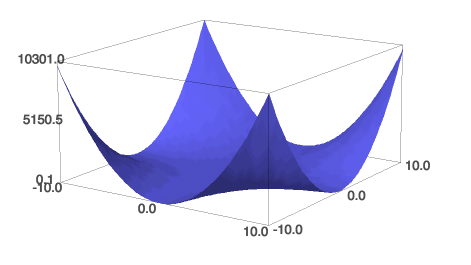
\includegraphics[width=0.8\textwidth]{plots/ch1_03_f(x,y).png}
				\caption{$f(x, y) = (xy - 1)^2 + x^2$.\label{fig:f(x,y)}}
			\end{center}
		\end{figure}
		
		Now, even if it holds, it does not help to obtain $\Qu$ at all:
		
		\begin{remark}
			There is no polynomial map 
			$$f(P_1, P_2): \R^2 \longrightarrow \R^2$$
			satisfying $f(\R^2) = \Qu$ and $P_1(x, y) = (xy - 1)^2 + x^2$.
		\end{remark}
		The proof of this remark uses the Curve Selection Lemma (\cite{abr}, VIII.2.6) to approach a point $(\lambda^2, 0) \in \overline{\Qu}$ with $\lambda > 0$, to get a contradiction.
		
		On the topic of finding a polynomial map $\Phi: \R^2 \longrightarrow \R^2$ that satisfies $\Phi(\R^2) = \Qu$, the mayor difficulty is:
		
		\begin{center}
			\begin{tabular}{rr}
				$\qquad \ \, $ \fbox{\textit{The closure of its image contains the positive half-axes.}} & $\quad$ ($\clubsuit$)
			\end{tabular}
		\end{center}
		
		\begin{remark}
			Using theorem \ref{finSetTh}, we just need to find a polynomial map $$\P = (\F, \G): \R^2 \longrightarrow \R^2$$ such that $\P(\R^2)$ is the disjoint union of $\Qu$ and a set with finite preimage, say $F \rightsquigarrow \P(\R^2) = \Qu\ \sqcup F$. This way we could apply the theorem and transform $\R^2$ into  $\R^2 \setminus F$ with a map $\varphi$, and then use $\P$ to get $\Qu \rightsquigarrow\Phi = \P \circ \varphi$. 
		\end{remark}
		
		We are going to give a map $\P = (\F , \G)$ that accomplish this task, with $F$ being the set $\set{(-1, 0), (0, -1)}$. If we are able to find such $\P$, then ($\clubsuit$) will immediately be satisfied. 
		
		Thus, for every $\lambda, \mu \ge 0$ there will exist \hyperref[curveGerms]{analytic half branch curve germs} $\alpha_{\lambda}(s),\beta_{\mu}(s)$ which cannot be extended to $0$ and such that:
		$$
		\lim_{s\rightarrow 0} P(\alpha_{\lambda}(s))=(\lambda^2,0)\qquad \text{and} \qquad
		\lim_{s\rightarrow 0} P(\beta_{\mu}(s))=(0,\mu^2).
		$$
		We can try parametrizations like:
		$$
		\alpha_{\lambda}(s)=\left(s^{n_{\lambda}},\frac{a_{\lambda 0}+a_{\lambda 1}s+\cdots}{s^{m_{\lambda}}}\right)
		\quad \text{ and } \quad
		\beta_{\mu}(s)=\left(\frac{b_{\mu 0}+b_{\mu 1}s+\cdots}{s^{\ell_{\mu}}},s^{k_{\mu}}\right).
		$$
		Then $a_{\lambda 0},b_{\mu 0}$ must be constants (except maybe for finitely many values of $\lambda$ and $\mu$). In view of this, we will take curves of the type:
		$$
		\alpha_{\lambda}(s)=\left(s^{n_{\lambda}},\frac{1+a_{\lambda 1}s+\cdots}{s^{m_{\lambda}}}\right)
		\quad \text{ and } \quad
		\beta_{\mu}(s)=\left(\frac{1+b_{\mu 1}s+\cdots}{s^{\ell_{\mu}}},s^{k_{\mu}}\right),
		$$
		and we can choose the simplest possible curves:
		$$
		\alpha_{\lambda}(s)=\left(s,\frac{1+a_{\lambda }s}{s}\right)
		\quad \text{ and } \quad
		\beta_{\mu}(s)=\left(\frac{1+b_{\mu }s}{s},s^{3}\right).
		$$
		
		The following pair of polynomials:
		
		\begin{equation*}
			\boxed{
				\begin{aligned}
					\F(x, y) & = (1 - x^3 y + y - x y^2)^2 + (x^2 y)^2 & = &\  \F_1^2 + \F_2^2 \\
					\G(x, y) & = (1 - xy + x - x^4 y)^2 + (x^2 y)^2 & = &\ \G_1^2 + \G_2^2\\
				\end{aligned}
			}
		\end{equation*}
		
		have a good behavior along these curves, meaning:
		
		\begin{figure}[h]\hspace{-0.5cm}
			\begin{subfigure}{.54\linewidth}\centering
				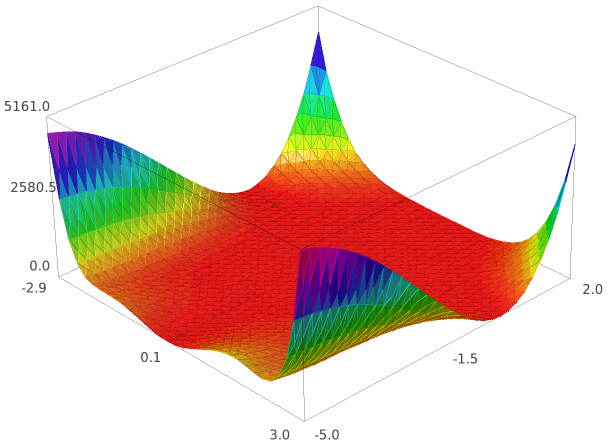
\includegraphics[width=1\textwidth]{plots/ch1_04_F.png}
				\caption{$\F(x, y) = (1 - x^3 y + y - x y^2)^2 + (x^2 y)^2$.\label{fig:F}}
			\end{subfigure}
			\begin{subfigure}{.55\linewidth}\centering
				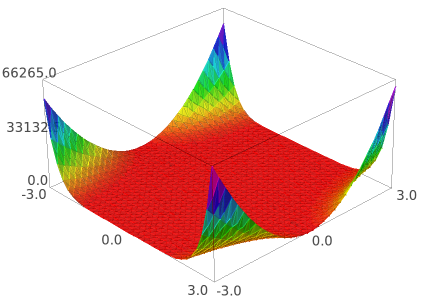
\includegraphics[width=1\textwidth]{plots/ch1_05_G.png}
				\caption{$\G(x, y) = (1 - xy + x - x^4 y)^2 + (x^2 y)^2$.\label{fig:G}}
			\end{subfigure}\\[1ex]
			\caption{Plots of the polynomials $\F, \G: \R^2 \longrightarrow \R$.\label{fig:plotFG}}
		\end{figure}
		
		\begin{enumerate}[(a)]
		
			\item $\cdot$ $\F_1 \circ \alpha_\lambda = 1 -a_{\lambda}-a_{\lambda}^{2} s-s^{2}-a_{\lambda} s^{3} \in \R[s,a_{\lambda}]$.
			
				$\ \ \F_1\circ\alpha_{\lambda }(0)=1-a_{\lambda }$.
			
				$\cdot$ $\F_1\circ\beta_{\mu} = -3 \, b_{\mu} s - 3 \, b_{\mu}^{2} s^{2} - {\left(b_{\mu}^{3} - 1\right)} s^{3}-s^{5}-b_{\mu}s^{6} \in\R[s,b_{\mu}]$.
				
				$\ \ \F_1\circ\beta_{\mu}(0)=0$.
				
			\item $\cdot$ $ \G_1\circ\alpha_{\lambda } = {\left(1-a_{\lambda} \right)} s -s^{3} -a_{\lambda} s^{4} \in\R[s,a_{\lambda}]$.
			
				$\ \ \G_1\circ\alpha_{\lambda }(0)=0$.
			
				$\cdot$ $\G_1\circ\beta_{\mu} = 1-3 \, b_{\mu}-6 \, b_{\mu}^{2} s-{\left(4 \, b_{\mu}^{3} + 1\right)} s^{2}-{\left(b_{\mu}^{4} + b_{\mu}\right)} s^{3} \in\R[s,b_{\mu}]$.
				
				 $\ \ \G_1\circ\beta_{\mu}(0)=1-3b_{\mu}$.
		
			\item $\cdot$ $\F_2\circ\alpha_{\lambda }= s+a_{\lambda} s^{2} = \G_2\circ\alpha_{\lambda}\in\R[s,a_{\lambda }]$.
			
				$\cdot$ $\F_2\circ\beta_{\mu}= s+2 \, b_{\mu} s^{2}+b_{\mu}^{2} s^{3} = \G_2\circ\beta_{\mu}\in\R[s,b_{\mu}]$.
				
				$\cdot$ $\F_2\circ\alpha_{\lambda }(0)=\G_2\circ\alpha_{\lambda}(0)=\F_2\circ\beta_{\mu}(0)=\G_2\circ\beta_{\mu}(0)=0$.
		
		\end{enumerate}
		
		All of these map compositions were computed by Sage. Thus, we get these properties:
		
		\begin{enumerate}[(i)]
		
			\item The polynomials $\F, \G$ are non-negative in $\R^2$.
		
			\item $\cdot$ $\F^{-1}(0)=\F_1^{-1}(0)\cap \F_2^{-1}(0)= \{(0,-1)\} \xmapsto{\ \P\ } \set{(0,1)}$.
			
				 $\cdot$ $\G^{-1}(0)=\G_1^{-1}(0)\cap \G_2^{-1}(0)\ =\, \{(-1,0)\} \xmapsto{\ \P\ } \set{(1,0)}$.
		
			\item $\cdot$ $P\circ\alpha_{\lambda}=(F\circ\alpha_{\lambda },G\circ\alpha_{\lambda})=$
			
				$\arraycolsep=2pt\def\arraystretch{1.2}
				\begin{array}{l}
					\left(\right.a_{\lambda}^{2}-2 \, a_{\lambda}+1+2 \, {(a_{\lambda}^{3} - a_{\lambda}^{2})} s+{(a_{\lambda}^{4} + 2 \, a_{\lambda} - 1)} s^{2}+4 \, a_{\lambda}^{2} s^{3}+\\
					\quad {(2 \, a_{\lambda}^{3} + a_{\lambda}^{2} + 1)} s^{4}+2 \, a_{\lambda} s^{5}+a_{\lambda}^{2} s^{6},	\\		
					\ {(a_{\lambda}^{2} - 2 \, a_{\lambda} + 2)} s^{2}+2 \, a_{\lambda} s^{3}+{(a_{\lambda}^{2} + 2 \, a_{\lambda} - 2)} s^{4} + \\
					\quad \, 2 \, {(a_{\lambda}^{2} - a_{\lambda})} s^{5}+s^{6}+2 \, a_{\lambda} s^{7}+a_{\lambda}^{2} s^{8}\left.\right).
				\end{array}
				$
				
				$\cdot$ $P\circ\beta_{\mu}=(F\circ\beta_{\mu},G\circ\beta_{\mu})=$
				
				$\arraycolsep=2pt\def\arraystretch{1.2}
				\begin{array}{l}
					\left(\right.{(9 \, b_{\mu}^{2} + 1)} s^{2}+2 \, {(9 \, b_{\mu}^{3} + 2 \,b_{\mu})} s^{3}+3 \, {(5 \, b_{\mu}^{4} + 2 \, b_{\mu}^{2} - 2 \, b_{\mu})}s^{4}+\\
					\quad 2 \, {(3 \, b_{\mu}^{5} + 2 \, b_{\mu}^{3} - 3 \, b_{\mu}^{2})}s^{5}+{(b_{\mu}^{6} + b_{\mu}^{4} - 2 \, b_{\mu}^{3} + 6 \, b_{\mu} + 1)} s^{6}+\\
					\quad 12 \,b_{\mu}^{2} s^{7}+2 \, {(4 \, b_{\mu}^{3} - 1)} s^{8}+2 \, {(b_{\mu}^{4} -b_{\mu})} s^{9} + s^{10} + 2 \, b_{\mu} s^{11}+b_{\mu}^{2} s^{12},\\
					\ 9 \, b_{\mu}^{2}-6 \, b_{\mu}+1+12 \, {(3 \, b_{\mu}^{3} - b_{\mu}^{2})} s+{(60\, b_{\mu}^{4} - 8 \, b_{\mu}^{3} + 6 \, b_{\mu} - 1)} s^{2} + \\
					\quad 2 \, {(27 \, b_{\mu}^{5}- b_{\mu}^{4} + 9 \, b_{\mu}^{2} + b_{\mu})} s^{3}+{(28 \, b_{\mu}^{6} + 20 \, b_{\mu}^{3}+ 6 \, b_{\mu}^{2} + 1)} s^{4}+\\
					\quad 2 \, {(4 \, b_{\mu}^{7} + 5 \, b_{\mu}^{4} + 2\, b_{\mu}^{3} + b_{\mu})} s^{5}+{(b_{\mu}^{8} + 2 \, b_{\mu}^{5} + b_{\mu}^{4} +b_{\mu}^{2})} s^{6}\left.\right).
					\end{array}
				$
					
		\end{enumerate}
		
		The polynomials $F\circ\alpha_{\lambda }, G\circ\alpha_{\lambda} \in \R[s,a_{\lambda}]$ and $F\circ\beta_{\mu},G\circ\beta_{\mu} \in\R[s,b_{\mu}]$ were computed with Sage. As we anticipated before, by (ii) $F = \set{(-1, 0), (0, -1)}$.
		
	\end{subsection}
	
	\begin{subsection}{The proof}
		
		\begin{Proof}(of theorem \ref{openQuad})
			
			We are going to prove that $\Qu \subset \P(\R^2)$, and to do this it is enough to fix $v > 0$, and if $\G = v$ then the image of $\F$ must contain the whole positive interval $(0, +\infty)$.
			\begin{center}
				\fbox{\textbf{Step 1}} \emph{Parametrization of the curve $\{\G-v=0\}$.}
			\end{center}

			We start by solving the equation $\G-v= 0 = (1 - xy + x - x^4 y)^2 + (x^2 y)^2 - v$. It has degree $2$ on $y$, so we obtain roots $y^+(x,v),\ y^-(x,v)$:
			\begin{equation*}
				\begin{aligned}
				y^+(x,v) & =\frac{1 + x + x^3 + x^4 + \sqrt{\Delta(x,v)}}{x(x^2 + (x^3 + 1)^2)}\\
				y^-(x,v) & =\frac{1 + x + x^3 + x^4 - \sqrt{\Delta(x,v)}}{x(x^2 + (x^3 + 1)^2)}\\
				\end{aligned}
			\end{equation*}
			where $\Delta(x,v) = \Delta_v(x):=v(x^2+(x^3+1)^2)-x^2(x+1)^2,\ \text{deg}_x(\Delta) = 6$. We can see on figure \ref{fig:plotYs_1} how $y^+$ and $y^-$ look like for instance for $v = 0.8$. As we can see on figure \ref{fig:plotYs_2}, for $v = 1$ there are no singularities on $y^-$. This observation is used later, in Step 2.
			
			\begin{figure}
				\centering
				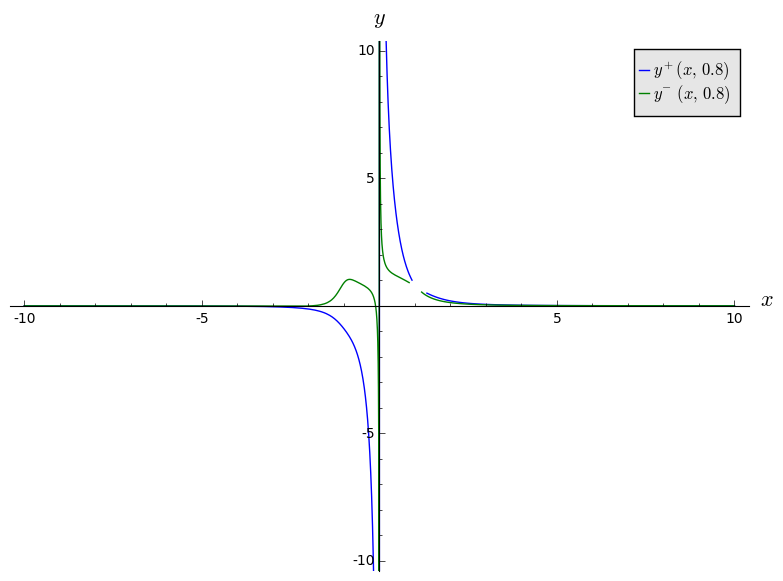
\includegraphics[width=1\textwidth]{plots/ch1_06_sols.png}
				\caption{$y^+(x,v)$ and $y^+(x,v)$ for $v = 0.8$.\label{fig:plotYs_1}}
			\end{figure}
			
			\begin{figure}
				\centering
				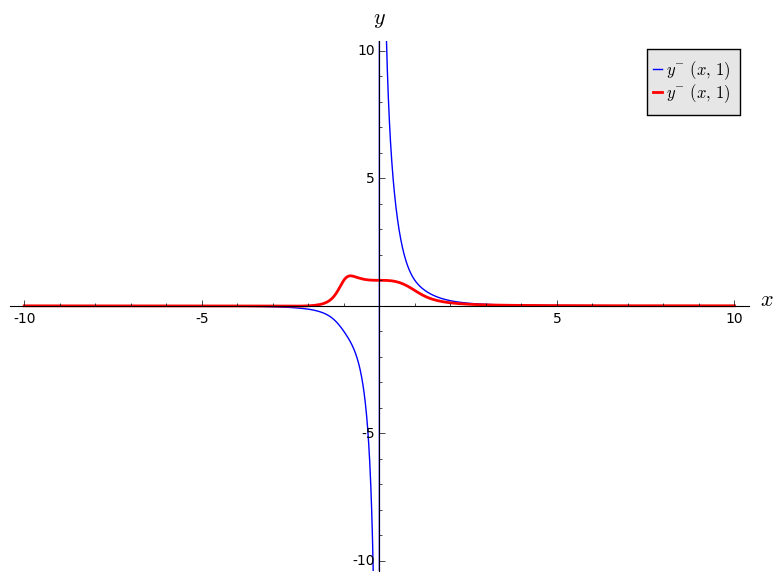
\includegraphics[width=1\textwidth]{plots/ch1_07_sols_1.png}
				\caption{$y^+(x,v)$ and $y^+(x,v)$ for $v = 1$.\label{fig:plotYs_2}}
			\end{figure}

			The common domain of these two functions is defined by $D_v=\{x \in \R :\ \Delta(x,v) \geq 0, x \neq 0\}$, notice that the only real root of the denominator is $x_0 = 0$\footnote{We did check with Laguerre's method (implemented with Python 2.7.) that $x^7 + 2x^4 + x^3 + x$ has 6 complex roots.}. Let
			$$\begin{matrix}
				\begin{aligned}
					\gamma_v^+: D_v & \longrightarrow \R\\
					x &\longmapsto \F(x,y^+(x,v))\\
					\end{aligned}
 				& \qquad
				\begin{aligned}
					\gamma_v^-:D_v & \longrightarrow \R\\
					x &\longmapsto \F(x,y^-(x,v))\\
				\end{aligned}
			\end{matrix}$$
			
			Notice that $\text{im}(\F(\set{\G = v})) = \text{im}(\gamma_v^+) \cup \text{im}(\gamma_v^-)$, so our aim is to prove that $\text{im}(\gamma_v^+) \cup \text{im}(\gamma_v^-) \supset (0, +\infty)$.
			
			\begin{center}
				\fbox{\textbf{Step 2}} \emph{Main properties of $\gamma_v^+ \text{ and } \gamma_v^-$.}
			\end{center}
			
			In this section we are going to prove that:
			$$\text{(i)} \lim_{x\rightarrow \pm\infty}\gamma_v^+(x)=\lim_{x\rightarrow \pm\infty}\gamma_v^-(x)=0.$$
			$$\text{(ii)} \lim_{x\rightarrow 0}\gamma_v^+(x)=+\infty
				,\quad 
				\lim_{x\rightarrow 0}\gamma_v^-(x) =
				\left\{\begin{array}{ll}
					+\infty & \text{ for $v\neq 1$}\\
					4 & \text{for $v=1$}
				\end{array} \right.
			$$

			With Sage, we can symbolically check how $\gamma_v^+ \text{ and } \gamma_v^-$ look like, getting polynomials $A_1,A_2,B_1,B_2\in\R[x,v]$ and $C\in \R[x]$ such that:
			$$\text{(a) } \gamma_v^+(x)=\dfrac{A_1(x,v)+B_1(x,v)\sqrt{\Delta(x,v)}}{C(x)}, \ \ 
			\gamma_v^-(x)=\dfrac{A_2(x,v)+B_2(x,v)\sqrt{\Delta(x,v)}}{C(x)}$$
			$$\text{(b)}\ \ 
				\arraycolsep=1.4pt\def\arraystretch{1.5}
				\begin{array}{cclr}
					A_1(x, v) & = &\ \ A_2(x, v)\, , & \text{deg}_x(A_1) = \text{deg}_x(A_2) = 24\\
					B_1(x, v) & = & - B_2(x, v)\, , & \text{deg}_x(B_1) = \text{deg}_x(B_2) = 21\\
					C(x) & = & x^2(x^2+(x^3+1)^2)^4\, , & \text{deg}_x(C) = 26
				\end{array}
			$$
			
			We proceed to study $\gamma_v^+$ and $\gamma_v^-$ at the origin. Since $\Delta$ has even degree and positive leading coefficient on $x$, it is positive for $\abs{x}$ large enough, so (i) holds.
			
			Now, for $x = 0$, we get $\Delta(0, v) = v > 0 \imp 0 \in \overline{D_v}$. Also:
			\begin{itemize}
				\item $A_1(0,v) + B_1(0,v) \sqrt{\Delta(0,v)} = v(1+\sqrt{v})^2 > 0$.
				
				\item $A_2(0,v) + B_2(0,v) \sqrt{\Delta(0,v)} = v(1-\sqrt{v})^2 \geq 0$, and it is $0$ $\siff v = 1$.
			\end{itemize}
			
			\begin{figure}[h]
				\centering
				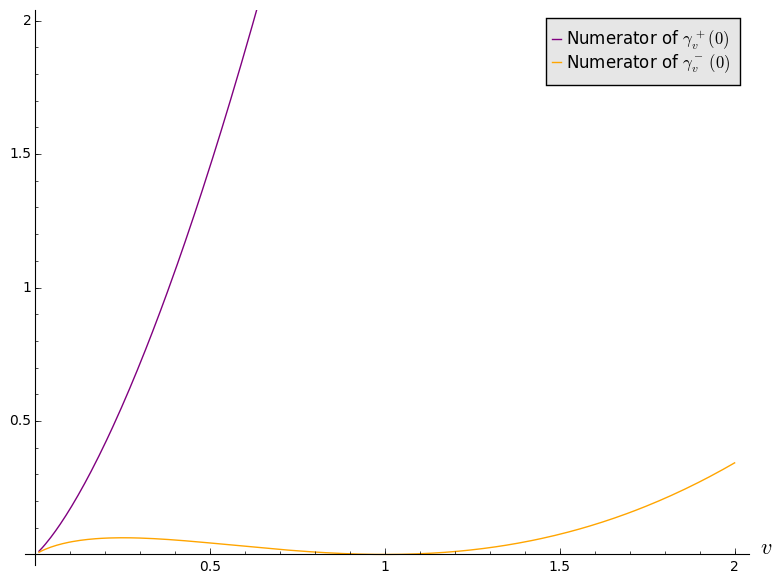
\includegraphics[width=0.65\textwidth]{plots/ch1_08_numerators.png}
				\caption{Numerators of $\gamma_v^+$ and $\gamma_v^+$ for $x = 0$.\label{fig:numerators}}
			\end{figure}
			
			Thus, (ii) holds (we also checked with Sage). The result for $v = 1$ on (ii) is not relevant here (see figure \ref{fig:limit}).
			
			\begin{figure}[h]
				\centering
				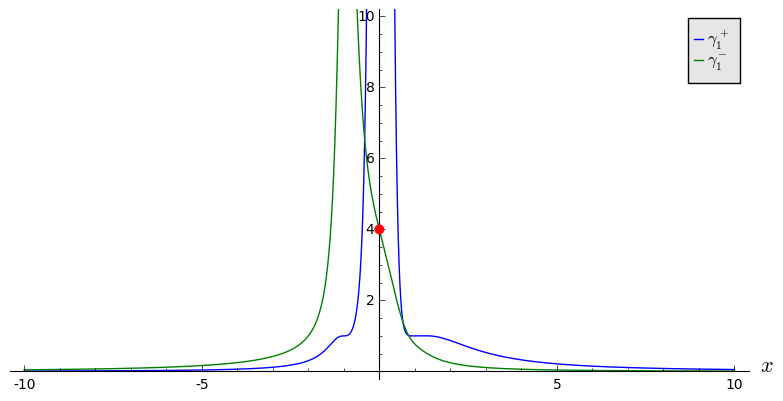
\includegraphics[width=1\textwidth]{plots/ch1_09_limit.png}
				\caption{Notice the value of $\gamma_1^-$ at $x = 0$.\label{fig:limit}}
			\end{figure}

			\begin{center}
				\fbox{\textbf{Step 3}} \emph{When $v \geq 0.28^2$ we have that} $\text{im}(\gamma_v^+) \supset (0, +\infty)$.
			\end{center}
			
			We are now going to study the domain $D_v$, in order to see whether $ (\gamma_v^+) \cup \text{im}(\gamma_v^-) \supset (0, +\infty)$ or not. Taking into account the definition of $D_v$, we need to study when $\Delta(x, v) = 0$, so it seems convinient to define:
			$$v(x)=\frac{x^2(x+1)^2}{x^2+(x^3+1)^2}$$
			%, whose graph can be seen in figure \ref{}.
			
			If $x \in (-\infty, 0)$, using Laguerre's method we checked that $\Delta(x, 0.28^2)$ has 4 complex roots and 2 real ones\footnote{The value $v_0 = 0.28^2$ comes from a careful observation of the plots figure \ref{}.}, with the real ones being $\delta_0 \approx 0.236$ and $\delta_1 \approx 4.336$. Thus, we get that when $v \ge 0.28^2$, $\Delta(x, v)$ has no negative roots, and moreover, it is positive $\imp (-\infty, 0) \subset D_v$. But then, since $\gamma_v^+$ is continuous and recalling the limits computed in Step 2, we get that $(0, +\infty) \subset \text{im}(\gamma_v^+) \subset \text{im}(\gamma_v^+) \cup \text{im}(\gamma_v^-)$.
			
			\begin{center}
				\fbox{\textbf{Step 4}} \emph{When $0 < v < 0.28^2$ we have that} $\text{im}(\gamma_v^-) \supset (0, +\infty)$.
			\end{center} 
			
			To prove that for $0 < v < 0.28^2$ we have that $(0, +\infty) \subset \text{im}(\gamma_v^-)$ it is enough to prove the existence of $N_v, \delta_v\in \R$ verifying			
			\begin{equation*}\qquad \quad
				\boxed{
					 N_v < \delta_v,\ \ (-\infty, N_v] \cup [\delta_v, +\infty) \subset D_v \text{ and } \gamma_v^-(N_v) > \gamma_v^+(\delta_v)\\
				}\qquad (\spadesuit)
			\end{equation*}
			%Incluir gráfica de lo que estamos diciendo con esta condicion
			
			To prove the existance of such $N_v$ and $\delta_v$, we must compute the roots of $\Delta_v(x)$ in the field of Puiseux series %incluir referencia en el apendice
			$\C\left(\set{v^*}\right)$, because $\overline{\R[x, v]} = \C\left(\set{v^*}\right) = \C\left(\set{x^*}\right)$. %<--- Entiendo yo, no?
			Such roots are power series in $\C\left(\set{w}\right)$ with $w = \sqrt{v}$, and we can take the most and the least negative roots of $\Delta_v$ in $\R\left(\set{v^*}\right)$ that makes the infinitesimal $v$ greater than 0, namely:
			
			\begin{equation*}\left\{
				\begin{split}
					\eta_v=&-\frac{1}{w}+1+w+w^2+\frac{5}{2}w^3+\cdots\\
					\xi_v=&-w-w^2-\frac{5}{2}w^3-6w^4+\cdots
				\end{split}\right.
			\end{equation*}
			
			Considering the infinitesimal $v$, it is clear that the first coefficient of the series is the most meaningful (order wise) $\imp \eta_v < \xi_v$. Thus, and to be able to make calculations, we need to find a finite number of coefficients of the series, and relevant ones. Let
			
			\begin{equation*}\left\{
				\begin{split}
					N_v=&-\frac{1}{w}+1+w+w^2=\eta_v-(\frac{5}{2}w^3+\cdots)<\eta_v\\
					\delta_v=&-w-w^2-\frac{5}{2}w^3=\xi_v-(-6w^4+\cdots)>\xi_v
				\end{split}\right.
			\end{equation*}
			
			We can check on Sage that $-\infty<N_v<\delta_v<0$ for $v \in (0, 0.28^2) \siff w \in (0, 0.28)$. Now we can focus on proving $(\spadesuit)$. Since $\Delta(N_{w^2}, w^2)$ and $\Delta(\delta_{w^2}, w^2)$ are positive for $w \in (0, 0.28)$, we get that $\N_v, \delta_v\in D_v$.
			
			For first part, let $D=\bigcup_{v>0} D_v=\bigcup_{v>0}\set{x\in \R: \Delta(x,v)\geq 0,x\neq 0}$. Its boundary is the union of the axis $x=0$ and the curve given by the equation 
			$$
			\Delta(x, v) = 0 \imp v(x)=\frac{x^2(x+1)^2}{x^2+(x^3+1)^2}
			$$
			. The latter graph $\left(x, v(x)\right)$ is over the axis $v = 0$. Then, $(-\infty, N_v]$ and $[\delta_v, 0)$ are contained in the interior of $D_v$ for $v\in (0, 0.28^2)$, because the curves $\set{(\delta_v, v): 0 < v < 0.28^2}$ and $\set{(N_v, v): 0 < v < 0.28^2}$ are contained in $D$, they are curves above the vertical axis $x = 0$, and $\delta_v < \xi_v$ and $N_v < \eta_v$ as we saw before. 
			
			So the only thing left to do is checking that $\gamma_v^-(N_v) > \gamma_v^-(\delta_v)$. Recall that 
			$$\gamma_v^-(x)=\dfrac{A_2(x,v)+B_2(x,v)\sqrt{\Delta(x,v)}}{C(x)}$$
			, with $\text{deg}_x(A_2) = 24, \text{deg}_x(B_2) = 21, \text{deg}_x(\Delta) = 6, \text{ and deg}_x(C) = 26$. Consider:
			
			$$
			\arraycolsep=2pt\def\arraystretch{1.5}
			\begin{array}{rclcrcl}
				\cdot\ f_1(w)&=&A_2(N_{w^2},w^2)\cdot w^{24}& \qquad &\cdot\ f_2(w)&=& A_2(\delta_{w^2},w^2)\\
				\cdot\ g_1(w)&=&B_2(N_{w^2},w^2)\cdot w^{21}& \qquad &\cdot\ g_2(w)&=&B_2(\delta_{w^2},w^2)\\
				\cdot\ q_1(w)&=&\Delta(N_{w^2},w^2)& \qquad &\cdot\ q_2(w)&=&\Delta(\delta_{w^2},w^2)\\
				\cdot\ h_1(w)&=&C(N_{w^2})\cdot w^{26}& \qquad &\cdot\ h_2(w)&=&C(\delta_{w^2})
			\end{array}
			$$
			. Consequently, we neew to prove that for $w \in (0, 0.28)$:
			$$
			\frac{f_1 \cdot (w^{24})^{-1} + g_1\cdot (w^{21})^{-1}\sqrt{q_1}}{h_1 \cdot (w^{26})^{-1}}
			> 
			\frac{f_2+g_2\sqrt{q_2}}{h_2} \iff
			$$

			$$
			\frac{w^2h_2f_1-f_2h_1}{h_1h_2}+\frac{w^5g_1\sqrt{q_1}}{h_1}-\frac{g_2\sqrt{q_2}}{h_2}>0
			$$

			, and we are going to prove that 
			$$
			\Lambda_1 := \frac{w^2h_2f_1-f_2h_1}{h_1h_2},\quad\Lambda_2 := \frac{w^5g_1\sqrt{q_1}}{h_1},\quad \Lambda_3 := -\frac{g_2\sqrt{q_2}}{h_2}
			$$
			are positive in the given interval, which only contains positive values. Thus and because $q_1, q_2$ are positive, we can clear away $w^5$ and $\sqrt{q_1}$ from $\Lambda_2$, $\sqrt{q_2}$ from $\Lambda_3$. Furthermore, $C(x) = x^2(x^2+(x^3+1)^2)^4 > 0$, so we can also remove $h_1$ and $h_2$ from $\Lambda_1, \Lambda_2, \Lambda_3$. It suffices to see that
			$$
			L:=\frac{w^2h_2f_1-f_2h_1}{w^4},\quad g_1,\quad K:=-\frac{g_2}{w^3}
			$$ 
			are positive for $w \in (0,0.28)$. 
			
			
			Thus, $(\spadesuit)$ holds and we have proved the result. \qed


		\end{Proof}
		
	\end{subsection}
	
\end{section}


\end{chapter}


\appendix
\begin{chapter}{Auxiliary definitions and results}

\begin{definition}\label{realCField}
	A \textbf{real closed field} is a field $R$ that has the $1\textsuperscript{st}$ order properties as the field of real numbers $\R$.
\end{definition}

\begin{definition}\label{semialgSet}
	A \textbf{semialgebraic set} is a subset $S \subset R^n$ (for some real closed field $R$) defined by a finite sequence of polynomial equations of the form:
	\begin{equation*}
	\left\{
	\begin{aligned}
		P_1(x_1,\, .\,&.\,.\, , x_n) = 0\\
		&\vdots\\
		P_r(x_1, .\,&.\,.\, , x_n) = 0 \\
		Q_1(x_1, .\,&.\,.\, , x_n) > 0 \\
		&\vdots\\
		Q_l(x_1, .\,&.\,.\, , x_n) > 0 \\
	\end{aligned}
	\right.
	\end{equation*}
	A \textbf{semialgebraic map} is a map that has semialgebraic graph. Moreover, the finite union, intersection and complement of semialgebraic sets is still a semialgebraic set.
\end{definition}

\begin{definition}[Zariski topology]\label{zariski}
	It is a topology on algebraic varieties whose closed sets are the algebraic subsets of the variety. Its sets are defined as the set of solutions of a system of polynomial equations over a field $R$. In this topology, when we talk about the irreducibility of an element, we mean that it is not the union of two smaller sets that are closed under the Zariski topology.
\end{definition}

\begin{definition}\label{pureDim}
	A set $S \subset R^n$ is said to be \textbf{pure dimensional} if its irreducible components are of the same dimension.
\end{definition}

\begin{definition}\label{properMap}
	A map $f$ is called \textbf{proper} if the preimage of every compact set is compact. A semialgebraic map $f: f^{-1}(K) \longrightarrow K$ is called \textbf{semialgebraically proper} if the preimage $f^{-1}(C)$ of a compact and semialgebraic subset $C \subset K$ is compact. This condition is weaker than the previous one.
\end{definition}

\begin{definition}\label{dominant}
	A polynomial map is said to be \textbf{dominant} if it has a dense image. 
\end{definition}

\begin{definition}\label{curveGerms}
	An \textbf{analytic half-branch curve germ} (\cite{bcr}, VII.4) is ... 
	%No se definirlo de manera formal, ni qué nivel de detalle alcanzar
\end{definition}

\end{chapter}


\begin{thebibliography}{10}

\bibitem[FerGam]{fg} J.F. Fernando, J.M. Gamboa: Polynomial images of $R^n$.
\textit{Journal of Pure and Applied Algebra}, {\bf 179}, (2003), no. 3, 241-254.

\bibitem[FerUen]{fu} J.F. Fernando, C. Ueno: A short proof for the open quadrant problem.
\textit{Preprint RAAG} (2014, submitted to MEGA 2015), 8 pages.

\bibitem[FeGaUe]{fgu} J.F. Fernando, J.M. Gamboa, C. Ueno: The open quadrant problem:
A topologycal proof. \textit{Preprint} (2015), 13 pages.

\bibitem[AnBrRz]{abr} C. Andradas, L. Br\"ocker, J.M. Ruiz: Constructible 
sets in real geometry.  \em Ergeb.  Math.  \em {\bf 33}.  Berlin Heidelberg 
New York: Springer Verlag, 1996.

\bibitem[BoCoRo]{bcr} J. Bochnak, M. Coste, M.-F. Roy: G\'eom\'etrie
alg\'ebrique r\'eelle. {\em Ergeb. Math. 12}, Springer-Verlag,
Berlin Heidelberg New York (1987).

\bibitem[G]{g} J.M. Gamboa: Reelle algebraische Geometrie, June,
$10^{\text{th}}-16^{\text{th}}$ (1990), \textit{Oberwolfach}.

\end{thebibliography}

\end{document}